\chapter{Einleitung}
In der heutigen Zeit gibt es viele interessante Gadgets, die unterschiedlichste Daten liefern. Seien das Pulsmesser, Heizungsregler oder das Multimediasystem zu Hause, diese Technologien lassen sich auch für den Fahrradfahrer nutzen. Es gibt bereits sogenannte Fahrradcomputer, welche die Geschwindigkeit messen und über ein separates Display ausgeben, jedoch werden die meisten mit einer Batterie betrieben, deren Laufzeit begrenzt ist. Mit der Möglichkeit des Energy Harvesting wird die Batterie und deren begrenzte Laufzeit gänzlich ersetzt. Bluetooth Low Energy kann Daten mit sehr wenig Energie übertragen, damit können die Daten, wie Geschwindigkeit oder Höhenmeter, an ein Android-Endgerät übermittelt werden.


\section{Ausgangslage}

Stand der Technik: Geschwindigkeitsanzeige für Velofahrer aktuelle Beispiele beschreiben.

Zwei Nachteile: Batteriewechsel und zusätzliches Display. Ein Handy hat jeder. Deshalb diese zur Anzeige benutzen.



Vorarbeiten auf diesem Gebiet:
Roman Scheider und Daniel Studer verfassten 2015 eine Projektarbeit am InES, in der sie die Machbarkeit eines Bicyle computer and sensoric powerd with energy nachwiesen \cite{PA_bicycle}. 
Die Punkte, die sich zu unser Arbeit unterscheiden benennen.

Nennen, was in dieser Arbeit \textbf{neu} erarbeitet wird.
...



\section{Definition der Aufgabenstellung}
Überleitung:Aufgrund STand der Technik, folgende Aufgabenstellung gebaut (Ist ev.Abschlusssatz Stand der Technik).

In der Ausschreibung der Arbeit ist der Inhalt der Bachelorarbeit zusammengefasst (siehe \ref{anhang_ausschreibung}). Das Ziel der Arbeit besteht darin, einen bestehenden Prototypen eines batterielosen Fahrradcomputers zu verbessern und zu optimieren. Die bestehende Hardware soll optimiert und bestenfalls verkleinert werden. Weiter soll eine App für ein Android-Endgerät entwickelt werden, in der die Messwerte dargestellt werden.

Aus den Themen entstand eine Aufgabenstellung mit folgenden Punkten:


% [label={\alph*)}]
\begin{enumerate} 

\item Inbetriebnahme des Prototypen, Einlesen in die vorangegangene Projektarbeit und Beschäftigung mit der Materie, sind die Hauptpunkte des ersten Schrittes.

\item Die bestehende Hardware muss verkleinert und überarbeitet werden. Dafür wird ein neues PCB entworfen, welches verschiedene vorhandene Platinen vereint.

\item Initialisierung der Bluetooth-Schnittstelle muss auf dem Android-Endgerät und der Hardware vorgenommen werden. Eine erste Bluetooth-Kommunikation zwischen der Hardware und der Applikationen ist implementiert.

\item Das bestehende Energiemanagement soll auf die Anwendung eines Fahrradcomputers optimiert werden.

\item Die Benutzeroberfläche der Android-Applikation soll benutzerfreundlich und optisch ansprechend gestaltet werden.

\item Die erfassten Messwerte der Geschwindigkeit und der aktuellen Höhe sollen über Bluetooth übermittelt werden.

\item	Die erfassten Daten sollen gespeichert und nur dann übertragen werden, wenn die nötige Energie vorhanden ist.

\item	Per GPS soll die aktuelle Position ermittelt, sowie die bereits abgefahrene Route erfasst werden. Alles soll auf einer Karte veranschaulicht werden.

\item	Die Beschleunigung, Luftfeuchtigkeit und Temperatur sollen ebenfalls erfasst und über Bluetooth übermittelt werden.


\item	Das Energiemanagement soll für verschiedene Geschwindigkeiten optimiert werden.
\end{enumerate}

Für diese Bachelorarbeit sind die Punkte a) bis f) als Minimalanforderungen zu verstehen, während sich die Punkte f) bis j) dynamisch und in Abhängigkeit des Projektfortschritts gestalten lassen.


Aus diesen Anforderungen entstand der im Anhang \ref{anhang_projektplan} abgelegte Projektplan. 






\section{Übersicht der Aufgabenblöcke}
Aus der Aufgabenstellung sind folgende Arbeitsblöcke (siehe Abbildung \ref{arbeitsbloecke} ) entstanden. Die gepunkteten Blöcke sind optional, die voll umrandeten das Minimum. Die Projektplanung ist so aufgebaut, dass bei Meilenstein 1, das Layout gezeichnet ist, bei Meilenstein 2 die Kommunikation zur App besteht, bei Meilenstein 3 die überarbeitete Version des Prototyps gezeigt wird und bis dahin das Minimum erreicht ist. Welche optionalen Ziele realisiert werden, wird im Meilenstein 3 definiert. Der Projektplan findet sich im Anhang \ref{anhang_projektplan}.

\begin{figure}[h]
    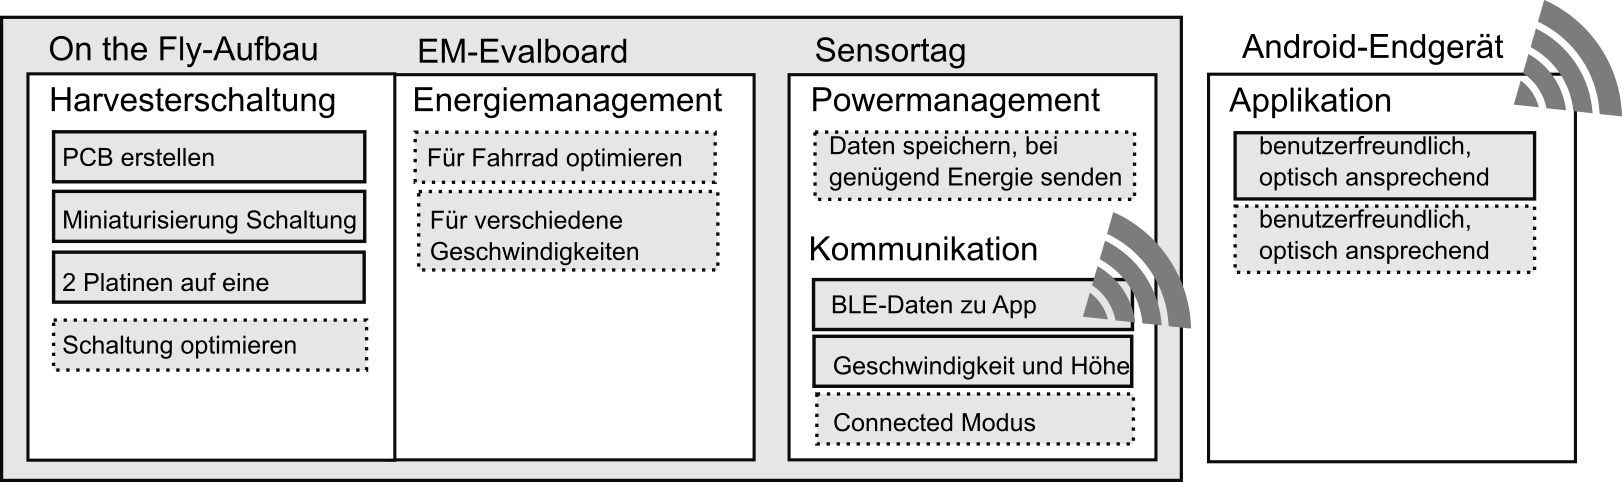
\includegraphics[scale=0.5]{../ressources/Projektorganisation/Arbeitsbloecke.png} 
    \caption{Arbeitsblöcke}
\end{figure}\label{arbeitsbloecke} 

